\documentclass[12pt]{article}
\usepackage[utf8]{inputenc}
\usepackage{amsmath, amssymb}
\usepackage{graphicx}
\usepackage{hyperref}
\usepackage{listings}
\usepackage{xcolor}
\usepackage{geometry}
\geometry{margin=1in}

\title{Entropy-Regularized Autoencoder}
\author{Hassan El Bouz}
\date{\today}

\definecolor{codebg}{rgb}{0.97,0.97,0.97}
\lstset{
  backgroundcolor=\color{codebg},
  basicstyle=\ttfamily\footnotesize,
  keywordstyle=\color{blue}\bfseries,
  commentstyle=\color{gray}\itshape,
  stringstyle=\color{orange},
  frame=single,
  breaklines=true,
  showstringspaces=false,
  columns=fullflexible
}

\begin{document}

\maketitle

\begin{abstract}
This report describes the implementation and analysis of an entropy-regularized autoencoder trained using PyTorch. The model aims to figure out the latent space by itself by incorporating both reconstruction loss and a custom entropic loss. We discuss the data pipeline, architecture, loss functions, training procedure, and experimental results, including interpretability of learned weights and latent codes.
\end{abstract}

\section{Introduction}
Autoencoders are unsupervised neural architectures designed to learn compact representations by reconstructing input data. While standard autoencoders minimize reconstruction error, their latent space is generally fixed with play over the structure of the latent space or interpretability. In this work, we enhance the autoencoder's capacity to learn to "compactify" the latent space by introducing an entropic regularization term.

\section{Theory and Background}
\subsection{Autoencoders}
Autoencoders are series of neural networks that encode input data into a lower-dimensional latent space and then decode it back to the original space. The architecture typically consists of an encoder, a bottleneck (latent space), and a decoder. The latent space has less neurons than the input, forcing the model to reduce the degrees of freedom (or better, dimension), thus learning a compressed representation of the input data. The output has the same shape as the input, and the model is trained by minimizing the difference between the input and output, usually using Mean Squared Error (MSE).

\subsection{Shannon Entropy}
Entropy, or Shannon Entropy, is a measure of uncertainty or randomness in a system. A generally good interpretation of entropy is the expected number of bits needed to encode the output of a random variable in the most efficient way, or an asymptotic limit. For example, if my random variable takes 4 values with equal probability, say, (A, B, C, D), the entropy is 2 bits, because I can encode each value with 2 bits (00 for A, 01 for B, 10 for C, and 11 for D). However, if A happens more frequently than the others, say with probability 0.50, the entropy will be lower, as I can encode A with 1 bit (0) and the others with 2 bits (11 for B, 100 for C, and 101 for D), and my expected number of bits will be lower than 2 bits. 

Entropy is defined mathematically as:
\[H(X) = -\sum_{i=1}^{n} p_i \log(p_i)\]
where \(p_i\) is the probability of the \(i\)-th outcome of a random variable \(X\). When we use logarithm base 2, it has units of bits, but any other logarithm differs by a constant multiple.
It is not difficult to prove that the maximum entropy is achieved when all outcomes are equally likely, i.e., \(p_i = \frac{1}{n}\) for \(n\) outcomes, and minimized when one outcome has probability 1 and all others have probability 0. In other words, the more my distribution is clustered, the lower the entropy. For uniform distributions, the entropy will simply be \(\log(n)\), where \(n\) is the number of outcomes.

\subsection{Renyi Entropy}
Renyi entropy is a generalization of Shannon entropy, defined as:
\[H_\alpha(X) = \frac{\alpha}{1-\alpha} \log \left(|| p ||_\alpha\right)\]
where \(|| \cdot ||_\alpha\) is \(\alpha-\)norm. 

A few special cases of Renyi entropy are:
\begin{itemize}
    \item For \(\alpha = 1\), it reduces to Shannon entropy.
    \item For \(\alpha = 0\), it reduces to the logarithm of the number of nonzero probabilities.
    \item For \(\alpha \to \infty\), it approaches the min-entropy, which is the negative logarithm of the maximum probability of any single outcome.
\end{itemize}

The intuition of Renyi entropy is that it generalizes the "logarithm of number of outcomes". Hence, the higher the \(\alpha\), the more it focuses on the most probable outcomes, while lower \(\alpha\) values consider all outcomes more equally.

\subsection{Entropic Compactifier Regularization}

In this subsection, we introduce how entropy can be used to create bottlenecks throughout the autoencoder architecture. The idea is to penalize the model for having more neurons in the bottleneck. But how do we do that? We can start with a fixed latent space size, say 20 neurons, and then assign to each neuron a weight that determines how "active" it is. There are two ways to do this: either sum the magnitude of the contributions of the incoming connections from the previous layer and add the biases, or sum the contributions of the outgoing connections to the next layer and add the biases. The first has the intuition of "Ah, this node is important! let's contrubute to it more", while the second has the intuition of "Ah, this node is important! let's use it more".

After evalutating the "activeness" of each neuron, we would like them to be more localized in the latent space. We can treat the weight distribution as a probability distribution after normalizing it, and then compute its entropy. We would like to minimize it, and the parameter \(\alpha\) controls how much we want to penalize the model for having more neurons in the bottleneck.

\subsection{Path Entropic Loss}

Another approach with dealing with bottlenecks is to consider all possible paths from the first layer to the last. Each path can be represented as a sequence of weights and biases, and we can assign a "cummulative" weight to each path by multiplying the weights and biases along it. Similar to the previous approach, the more weights the path has, the more "active" it is. A bottleneck can be created by penalizing the model for having more active paths, i.e. we want to localize the weights and biases into fewer paths. We hope that this localization will be "nice" and fall into one layer, creating a bottleneck. To do so we can do the same approach and calculate the entropy of the path distributions. Unfortunately, this approach is computationally expensive and scales up quickly, but as an advantage, it figures out the bottleneck location and size by itself.

\section{Implementation}
\subsection{Entropic Compactifier Loss Function}
The code for the Entropic Compactifier Loss Function is implemented in Pytorch. In short, we define 3 types of functions:
\begin{enumerate}
    \item \textbf{Node Value Functions:} These compute the "activeness" of each node in the latent space by summing the absolute values of incoming or outgoing weights and adding the biases.
    \item \textbf{Entropy:} These compute the entropy of the normalized node values, either for left or right nodes.
    \item \textbf{Entropic Loss Function:} This computes the entropy of the system from both left and right nodes by joining the weights, or adding both entropies
\end{enumerate}

The code is given below:

\break

\begin{lstlisting}[language=Python,caption={Entropic Compactifier Loss Function}]

def node_right_value(W, B):
    return torch.sum(torch.abs(W), dim=1) + torch.abs(B) # Weights for the incoming connections (node to the right)

def node_left_value(W, B):
    return torch.sum(torch.abs(W), dim=0) + torch.abs(B) # Weights for the outgoing connections (node to the left)

def entropic_loss_right(W, B, alpha=1.0, beta = 1.0):
    right_values = node_right_value(W, B)
    normalized_values = right_values / torch.sum(right_values)
    if beta == 1.0:
        loss = -torch.sum(normalized_values * torch.log(normalized_values + 1e-10))
    else:
        loss = beta/(1-beta) * torch.log(torch.norm(normalized_values, p=beta) + 1e-10)
    return alpha * loss

def entropic_loss_left(W, B, alpha=1.0, beta = 1.0):
    left_values = node_left_value(W, B)
    normalized_values = left_values / torch.sum(left_values)
    if beta == 1.0:
        loss = -torch.sum(normalized_values * torch.log(normalized_values + 1e-10))
    else:
        loss = beta/(1-beta) * torch.log(torch.norm(normalized_values, p=beta) + 1e-10)
    return alpha * loss

def entropic_loss(W_l, W_r, B, alpha=1.0, beta=1.0): # Difference between this and cumm_entropic_loss is that this one computes the loss for both left and right nodes separately
    loss_l = entropic_loss_left(W_r, B, alpha, beta)
    loss_r = entropic_loss_right(W_l, B, alpha, beta)
    return loss_l + loss_r

def cumm_entropic_loss(W_l, W_r, B, alpha=1.0): # Difference between this and entropic_loss is that this one assigns the node weight from the left and right before computing the loss
    values = node_right_value(W_l, B) + node_left_value(W_r, B)
    normalized_values = values / torch.sum(values)
    loss = -torch.sum(normalized_values * torch.log(normalized_values + 1e-10))  # Add small constant to avoid log(0)
    return loss * alpha

\end{lstlisting}

\subsection{Path Entropic Loss Function}
The path entropic loss function is more complex and requires iterating through all possible paths in the network. To ensure it is optimized, we first define an array that contains all possible paths we want to work with. Since this does not change, we do it once and then use it as the input in the loss function.

Later on, by using the optimized torch slicing, we can cleverly compute the products of the sum of weights and biases along each path. Finally, we compute the entropy of the path distribution.


\begin{lstlisting}[language=Python,caption={Path Entropic Loss Function}]

def path_entropy_parallel(first_node, last_node, weight_list, bias_list=None, a=1, paths = None):
    device = weight_list[0].device

    if paths is None:
        sizes = [w.size(1) for w in weight_list] + [weight_list[-1].size(0)]
        grids = [torch.arange(s, device=device) for s in sizes]
        all_paths = cartesian_product_gpu(grids)

        # Only keep paths from first_node to last_node
        valid_mask = (all_paths[:, 0] == first_node) & (all_paths[:, -1] == last_node)
        selected_paths = all_paths[valid_mask]
    else:
        selected_paths = paths

    if selected_paths.size(0) == 0:
        return torch.tensor(0.0, device=device, requires_grad=True)

    num_paths = selected_paths.size(0)
    num_layers = len(weight_list)

    weights = torch.ones(num_paths, device=device)

    for i in range(num_layers):
        src_idx = selected_paths[:, i]
        tgt_idx = selected_paths[:, i + 1]

        # Apply weight
        W = weight_list[i]

        # Apply bias at current source node
        if bias_list is not None and bias_list[i] is not None:
            weights *= torch.abs(W[tgt_idx, src_idx]) + torch.abs(bias_list[i][tgt_idx])
        else:
            weights *= torch.abs(W[src_idx, tgt_idx])

    # Normalize and compute entropy
    abs_weights = weights.abs()
    total = abs_weights.sum()
    probs = abs_weights / (total + 1e-9)

    if a == 1:
        entropy = -torch.sum(probs * torch.log2(probs + 1e-9))
    else:
        entropy = a / (1 - a) * torch.log2(torch.norm(probs, p=a))

    return entropy, selected_paths

\end{lstlisting}


\section{Methodology}

\subsection{Data Loading}
We use the MNIST dataset of $28\times 28$ grayscale handwritten digits to try to create a program that can generate number figures. PyTorch's \texttt{torchvision.datasets} provides an efficient pipeline. Data is batched for training.

\subsection{Model Architecture}
The autoencoder architecture is as follows:
\begin{itemize}
    \item Input: Flattened $28\times 28$ image
    \item Encoder: Linear layers with ReLU activations, compressing to a latent dimension
    \item Bottleneck: Several layers with the same latent size, enabling information bottlenecking
    \item Decoder: Mirrors the encoder, reconstructing back to image shape
    \item Output: Sigmoid activation for pixel values in $[0,1]$
\end{itemize}

In this implementation, we do not seperate the network explicitly into an encoder and decoder. Remember that the goal is to let the network figure out the bottleneck by itself, so we do not need to specify it. However, we can still guide the network into encoder and decoder to make training more efficient. We expect the bottleneck to happen somewhere in the "extended latent space" where it is just a safe area for the network to place the bottleneck appropriately.

\begin{lstlisting}[language=Python,caption={Autoencoder Definition}]
class Autoencoder(nn.Module):
    def __init__(self, extended_latent_dim=20):
        super().__init__()
        self.autoencoder = nn.Sequential(
            nn.Flatten(),
            nn.Linear(28*28, 64), nn.ReLU(),
            nn.Linear(64, extended_latent_dim), nn.ReLU(),
            nn.Linear(extended_latent_dim, extended_latent_dim), nn.ReLU(),
            nn.Linear(extended_latent_dim, extended_latent_dim), nn.ReLU(),
            nn.Linear(extended_latent_dim, 64), nn.ReLU(),
            nn.Linear(64, 28*28), nn.Sigmoid(),
            nn.Unflatten(1, (1, 28, 28))
        )
\end{lstlisting}

\subsection{Loss Function}
The total loss combines:
\begin{itemize}
    \item \textbf{Reconstruction Loss:} Mean Squared Error (MSE) between input and output.
    \item \textbf{Entropic Loss:} Either of the two entropic losses defined earlier.
\end{itemize}
\[
\text{Total Loss} = \lambda_1 \cdot \text{MSE} + \lambda_2 \cdot \text{EntropicLoss}
\]

In the first experiment, we work with the compactifier with $\lambda_1 = 0.7$ and $\lambda_2 = 0.3$ in our experiments.

\begin{lstlisting}[language=Python,caption={Loss Computation}]
recon = model(batch)
criterion_loss = criterion(recon, batch)
eloss = entropic_loss(W_l, W_r, B, alpha=1.0, beta=0.04)
loss = criterion_term * criterion_loss + entropy_term * eloss
\end{lstlisting}

Above, we specify based on preference the Renyi-Entropy of parameter \(0.04\) (called \(\beta\), while \(\alpha\) is the logarithm base), since we wish to capitalize over the smallest weights as well.

\subsection{Training Procedure}
We train for 20 epochs using Adam optimizer. At each batch:
\begin{enumerate}
    \item Forward pass
    \item Compute losses
    \item Backpropagation and parameter update
    \item Optionally, print weight statistics for monitoring
\end{enumerate}

\section{Experiments and Results}
In this setup, we were able to reduce the latent space size to 10 neurons. 

\subsection{Reconstruction Quality (Compactifier)}
\begin{figure}[ht]
    \centering
    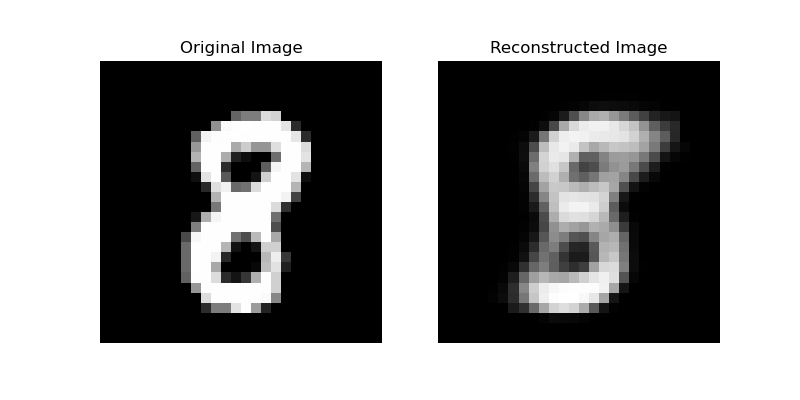
\includegraphics[width=0.4\textwidth]{recon_example.png}
    \caption{Sample reconstructed digits after training.}
\end{figure}

The encoding of the digits is:
\begin{verbatim}
[9.5884e-03, 0.0000e+00, 3.6991e+00, 0.0000e+00, 0.0000e+00, 0.0000e+00,
 3.0069e+01, 6.4067e+00, 4.2131e+01, 1.4036e-02, 2.1916e-02, 0.0000e+00,
 0.0000e+00, 1.2810e+02, 0.0000e+00, 5.8852e+00]
\end{verbatim}

Which, even though is of size 16, we use less than 10 neurons to encode it. The machine "deactivates" the neurons, but not remove them completely. Of course, we can rewrite the entire network with only these 10 neurons.

\subsection{Latent Space Analysis (Compactifier)}
To analyze what each neuron in the latent space does, we send to the decoder a tensor full of zeros except at a single neuron where we vary the value from -3 to 3. The decoder will then reconstruct the image, and we can see how each neuron affects the output.

\begin{figure}[ht]
    \centering
    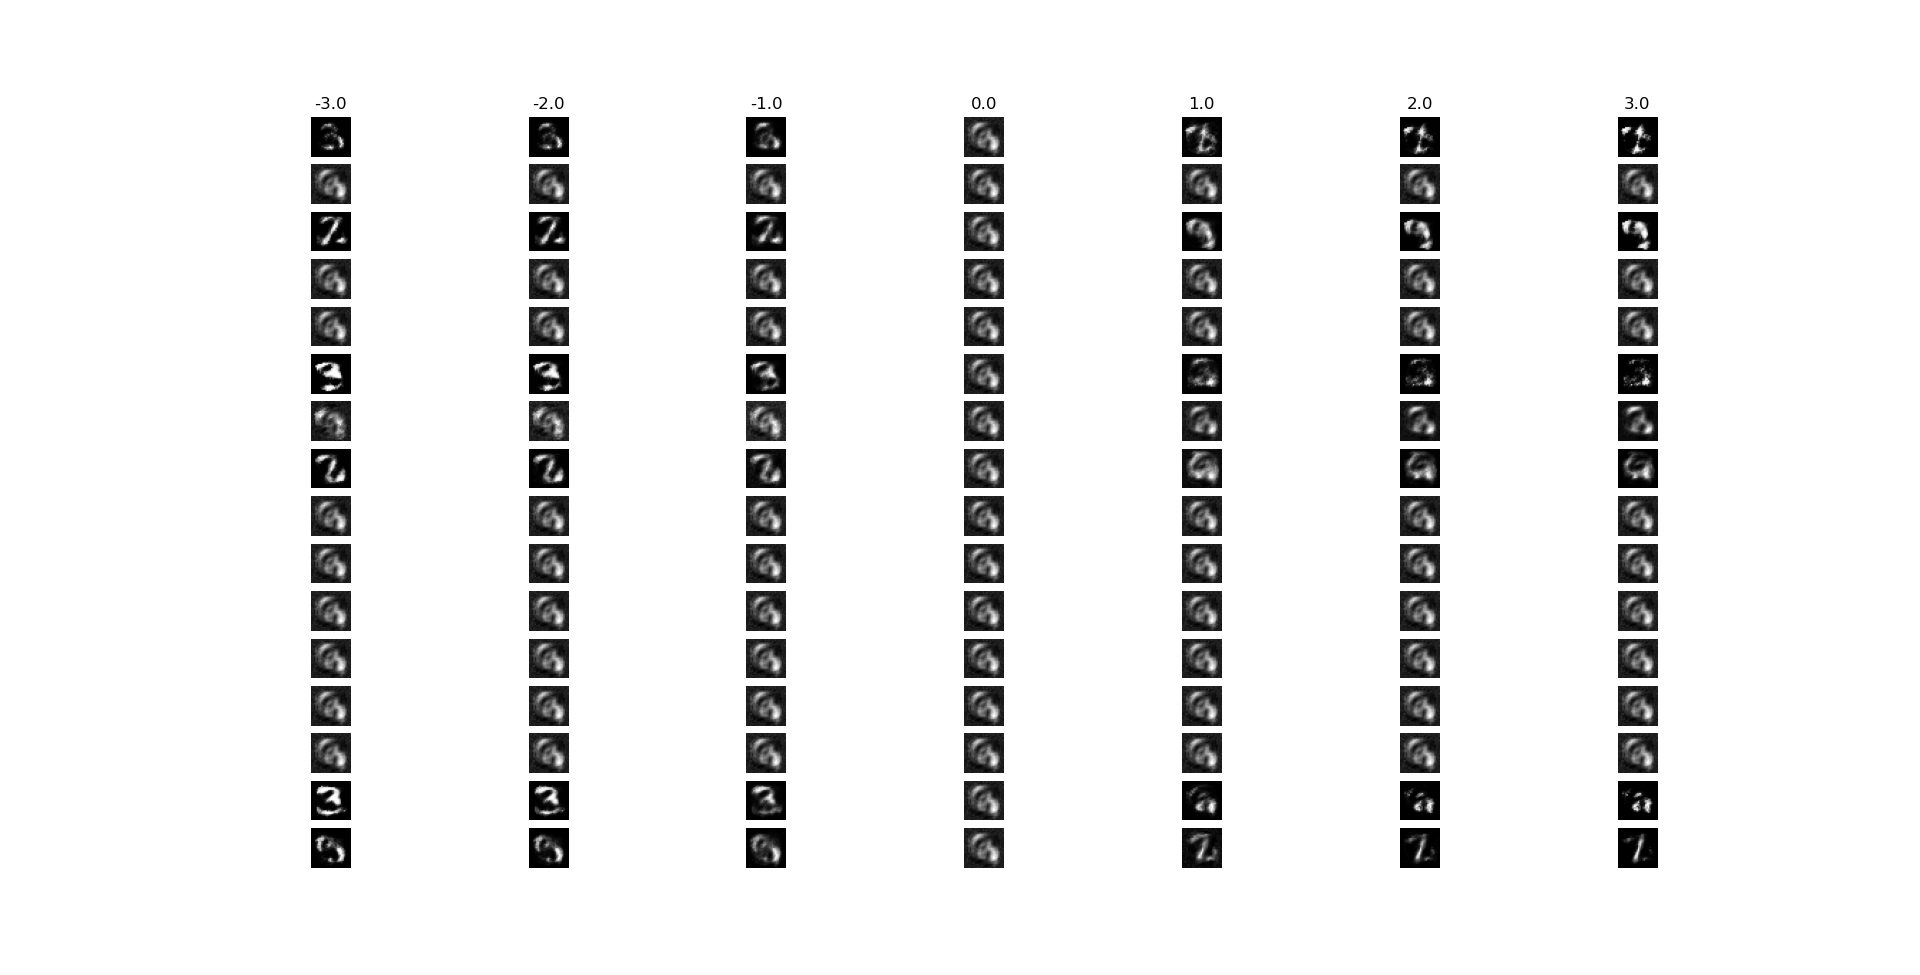
\includegraphics[width=1\textwidth]{latent_analyse.png}
    \caption{Sample reconstructed latent space after training.}
\end{figure}

We further see that some neurons do not play a role

\subsection{Reconstruction Quality (Path Entropic Loss)}

After training the autoencoder, we were able to achieve this latent structure:

\begin{verbatim}
Layer 0: 784 effective nodes (28*28 = 784)
Layer 1: 64 effective nodes
Layer 2: 16 effective nodes
Layer 3: 4 effective nodes
Layer 4: 12 effective nodes
Layer 5: 64 effective nodes
Layer 6: 784 effective nodes
\end{verbatim}

In this case, we were too extreme by reducing it to 4 neurons. Nevertheless, let us do the analysis of it.

\begin{figure}[ht]
    \centering
    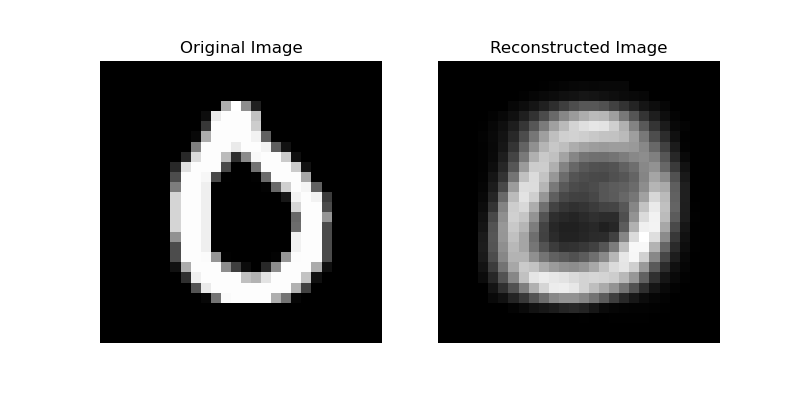
\includegraphics[width=0.4\textwidth]{recon_example_path.png}
    \caption{Sample reconstructed digits after path entropy training.}
\end{figure}

Things like 0, are encoded very well, but things like, 9, are encoded poorly.

\begin{figure}[ht]
    \centering
    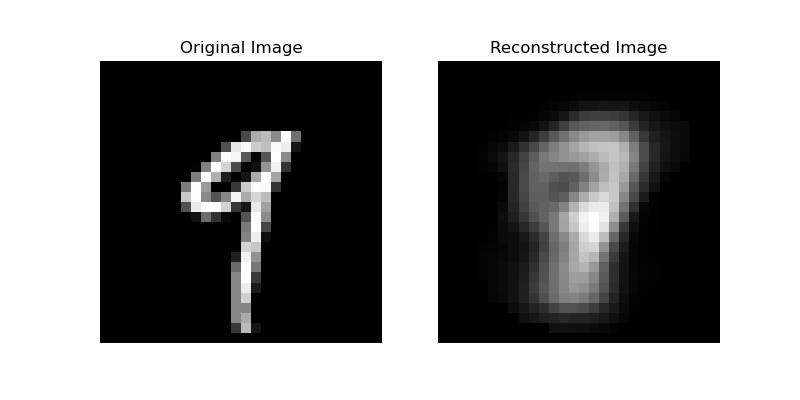
\includegraphics[width=0.4\textwidth]{recon_example_path_failed.png}
    \caption{Failed reconstructed digits after path entropy training.}
\end{figure}

To do the same analysis of the latent space as before, we send to the decoder a tensor full of zeros except at a single neuron where we vary the value from -3 to 3. The decoder will then reconstruct the image, and we can see how each neuron affects the output.

\begin{figure}[ht]
    \centering
    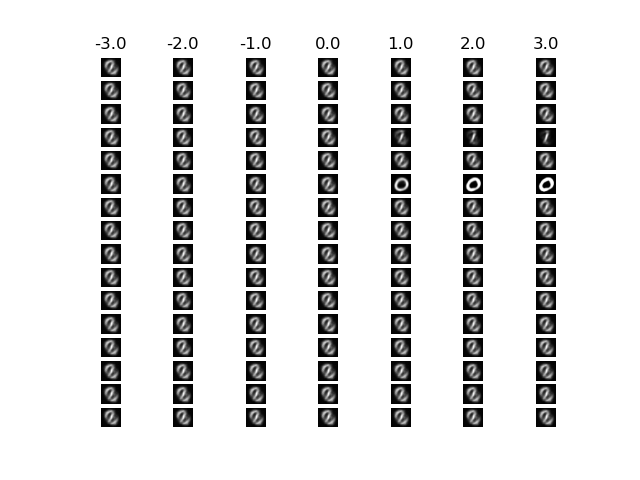
\includegraphics[width=1\textwidth]{latent_analyse_path.png}
    \caption{Sample reconstructed latent space after path entropy training.}
\end{figure}

\section{Adding Interpretability of Latent Space}
\subsection{Classifiers}
So far, the network compresses the images without any interpretability of the latent space, i.e. we do not know what each neuron does. To do so, we can attempt to assign meaning to each neuron by imposing a classification constraint. If the 784 pixel image is compressed to 8 neurons, we can add 10 neurons to the latent layer, and demand that these output the class of the image it belongs to. What we hope to achieve is that once we have the decoder, that takes \(8 + 10\) inputs, we can specify that we want to generate an image of the digit 3, and the initial 8 neurons will be filled with quantities that change the "handwriting" style.

This will be the first approach to letting a neural network "learn" the latent space that carries meaning, laying foundation to more complex constraints like Sindy or Sparcity. 

One layer of challenge we face is that we do not have control yet over the layer that will become the latent space. We can at every batch, scan each layer to determine the possible latent layer, and reserve the first 10 nodes for classification. 


\section{References}
\begin{itemize}
    \item \href{https://pytorch.org}{PyTorch documentation}
\end{itemize}

\end{document}
